\let\negmedspace\undefined
\let\negthickspace\undefined
\documentclass[journal]{IEEEtran}
\usepackage[a5paper, margin=10mm, onecolumn]{geometry}
%\usepackage{lmodern} % Ensure lmodern is loaded for pdflatex
\usepackage{tfrupee} % Include tfrupee package

\setlength{\headheight}{1cm} % Set the height of the header box
\setlength{\headsep}{0mm}     % Set the distance between the header box and the top of the text

\usepackage{gvv-book}
\usepackage{gvv}
\usepackage{cite}
\usepackage{amsmath,amssymb,amsfonts,amsthm}
\usepackage{algorithmic}
\usepackage{graphicx}
\usepackage{textcomp}
\usepackage{xcolor}
\usepackage{txfonts}
\usepackage{listings}
\usepackage{enumitem}
\usepackage{mathtools}
\usepackage{gensymb}
\usepackage{comment}
\usepackage[breaklinks=true]{hyperref}
\usepackage{tkz-euclide} 
\usepackage{listings}
% \usepackage{gvv}                                        
\def\inputGnumericTable{}                                 
\usepackage[latin1]{inputenc}                                
\usepackage{color}                                            
\usepackage{array}                                            
\usepackage{longtable}                                       
\usepackage{calc}                                             
\usepackage{multirow}                                         
\usepackage{hhline}                                           
\usepackage{ifthen}                                           
\usepackage{lscape}
\begin{document}

\bibliographystyle{IEEEtran}
\vspace{3cm}

\title{PHYSICS -2008}
\author{AI24BTECH11005 - Bhukya Prajwal Naik
}
% \maketitle
% \newpage
% \bigskip
{\let\newpage\relax\maketitle}

\renewcommand{\thefigure}{\theenumi}
\renewcommand{\thetable}{\theenumi}
\setlength{\intextsep}{10pt} % Space between text and floats


\numberwithin{equation}{enumi}
\numberwithin{figure}{enumi}
\renewcommand{\thetable}{\theenumi}


\begin{enumerate}
    

 
%16
    \item A circular disc of radius $a$ on the $x y$ plane has a surface charge density $\sigma=\frac{\sigma_{0} r \cos \theta}{a}$. The electric dipole moment of this charge distribution is
    \begin{multicols}{4}
			\begin{enumerate}
\item $\frac{\sigma_{0} \pi a^{4}}{4} \hat{x}$
\item $\frac{\sigma_{0} \pi a^{3}}{4} \hat{x}$
\item $-\frac{\sigma_{0} \pi a^{3}}{4} \hat{x}$
\item $-\frac{\sigma_{0} \pi a^{4}}{4} \hat{x}$
        \end{enumerate}
		\end{multicols}

%17
    \item At time $t=0$, a charge distribution $\rho(\vec{r}, 0)$ exists within an ideal homogeneous conductor of permittivity $\varepsilon$ and conductivity $\sigma$. At a later time $\rho(\vec{r}, t)$ is given by


		\begin{multicols}{1}
			\begin{enumerate}
	\item  $\rho(\vec{r}, t)=\rho(\vec{r}, 0) \exp \left(-\frac{\sigma t}{\varepsilon}\right)$
\item $\rho(\vec{r}, t)=\frac{\rho(\vec{r}, 0)}{1+(\sigma t / \varepsilon)^{2}}$
\item $\rho(\vec{r}, t)=\rho(\vec{r}, 0) \exp \left[-\left(\frac{\sigma t}{\varepsilon}\right)^{2}\right]$
\item $\rho(\vec{r}, t)=\rho(\vec{r}, 0) \frac{\varepsilon}{\sigma t} \sin \left(\frac{\sigma t}{\varepsilon}\right)$
			\end{enumerate}
		\end{multicols}

%18
    \item  A nonrelativistic charged particle moves along the positive $x$-axis with a constant positive acceleration $a \hat{x}$. The particle is at the origin at $t=0$. Radiation is observed at $t=0$ at a distant point $(0, d, 0)$ on the $y$-axis. Which one of the following statements is correct?
        
            \begin{enumerate}
             \item The radiation is unpolarized.
\item The radiation is plane polarized with polarization parallel to the $x$-axis.
\item The radiation is plane polarized with polarization parallel to the $x y$ plane along a line inclined to the $x$ axis.
\item The radiation is elliptically polarized.
            \end{enumerate}



      

%19
    \item For a physical system, two observables $\O_{1}$ and $O_{2}$ are known to be compatible. Choose the correct implication from amongst those given below:
		
			\begin{enumerate}
	\item Every eigenstate of ${O}_{1}$ must necessarily be an eigenstate of ${O}_{2}$.
\item Every non-degenerate eigenstate of ${O}_{1}$ must necessarily be an eigenstate of ${O}_{2}$.
\item When an observation of $O_{1}$ is carried out on an arbitrary state $|\Psi\rangle$ of the physical system, a subsequent observation of ${O}_{2}$ leads to an unambiguous result.
\item Observation of ${O}_{1}$ and ${O}_{2}$, carried out on an arbitrary state $|\Psi\rangle$ of the physical system, lead to the identical results irrespective of the order in which the observations are made.
	\end{enumerate}
		

%20 
    \item An exact measurement of the position of a simple harmonic oscillator (SHO) is made with the result $x=x_{0}$. [The SHO has energy levels $E_{n}(n=0,1,2, ....)$ and associated normalized wavefunctions $\psi_{n}$ ]. Subsequently, an exact measurement of energy $E$ is made. Using the general notation ${Pr}\left(E=E^{\prime}\right)$ denoting the probability that a result $E^{\prime}$ is obtained for this measurement, the following statements are written. Which one of the following statements is correct?
		\begin{multicols}{1}
			\begin{enumerate}
				
	\item ${Pr}\left(E=E_{0}\right)=0$
\item ${Pr}\left(E=E_{n}\right)=1$ for some value of $n$.
\item ${Pr}\left(E=E_{n}\right) \propto \psi_{{n}}(x)$
\item ${Pr}\left(E>E^{\prime \prime}\right)>0$ for any $E^{\prime \prime}$.
			\end{enumerate}
		\end{multicols}

%21
    \item Consider the combined system of proton and electron in the hydrogen atom in its (electronic) ground state. Let $I$ denote the quantum number associated with the total angular momentum and let $\alpha$ denote the magnitude of the expectation value of the net magnetic moment in the state. Which of the following pairs represents a possible state of the system ( $\mu_B$ is Bohr magneton)?
    \begin{multicols}{4}
            \begin{enumerate}
        \item $I=0,\alpha =0$
        \item $I=\frac{1}{2},\alpha =1\mu_B$
        \item $I=1,\alpha =1 \mu_B$
        \item $I=0,\alpha=2\mu_B$
        \end{enumerate}
        \end{multicols}
%22
    \item A particle is placed in a one dimensional box of size $L$ along the $x$-axis $(0<x<L)$. Which of the following is true?
    
            \begin{enumerate}
             \item In the ground state, the probability of finding the particle in the interval $(\frac{L}{4},\frac{3 L}{4})$ is half.
\item In the first excited state, the probability of finding the particle in the interval $(\frac{L}{4},\frac{3 L}{4})$ is half. This also holds for states with $n=4,6,8, ....$
\item For an arbitrary state $|\Psi\rangle$, the probability of finding the particle in the left half of the well is half.
\item In the ground state, the particle has a definite momentum. 
              \end{enumerate}
        
%23
    \item A calculator has accuracy up to 8 digits after decimal place. The value of $\int_{0}^{2 \pi} \sin x d x$ when evaluated using this calculator by trapezoidal method with 8 equal intervals, to 5 significant digits is
 \begin{enumerate}
	\item % Corrected Diagram (A) - Half ellipse reflected into the 4th quadrant
\begin{tikzpicture}
    % Axes
    \draw[->] (0,0) -- (0,2.5) node[left] {$p_z$};
    \draw[->] (0,-2.5) -- (0,0);
    \draw[dashed] (0,0) -- (3.5,0) node[below] {$z$};
    \draw[dashed] (-3.5,0) -- (0,0);
    \node at (0,0) [below left] {O};
    
    % Half ellipse (upper part in 1st quadrant)
    \draw[thick] (0,2) arc[start angle=90,end angle=0,x radius=3,y radius=2];
    
    % Reflection (lower part in 4th quadrant)
    \draw[thick] (0,-2) arc[start angle=270,end angle=360,x radius=3,y radius=2];
\end{tikzpicture}


	\item 
% Diagram (B) - Multiple ellipses reflected into the 4th quadrant with arrows
\begin{tikzpicture}
    % Axes
    \draw[->] (0,0) -- (0,2.5) node[left] {$p_z$};
    \draw[->] (0,-2.5) -- (0,0);
    \draw[dashed] (0,0) -- (3.5,0) node[below] {$z$};
    \draw[dashed] (-3.5,0) -- (0,0);
    \node at (0,0) [below left] {O};
    
    % Multiple ellipses (upper parts)
    \draw[thick] (0,2) arc[start angle=90,end angle=0,x radius=3,y radius=2];
    \draw[thick] (0,1.6) arc[start angle=90,end angle=0,x radius=2.5,y radius=1.6];
    \draw[thick] (0,1.2) arc[start angle=90,end angle=0,x radius=2,y radius=1.2];
    \draw[thick] (0,0.8) arc[start angle=90,end angle=0,x radius=1.5,y radius=0.8];
    
    % Reflections (lower parts in the 4th quadrant)
    \draw[thick] (0,-2) arc[start angle=270,end angle=360,x radius=3,y radius=2];
    \draw[thick] (0,-1.6) arc[start angle=270,end angle=360,x radius=2.5,y radius=1.6];
    \draw[thick] (0,-1.2) arc[start angle=270,end angle=360,x radius=2,y radius=1.2];
    \draw[thick] (0,-0.8) arc[start angle=270,end angle=360,x radius=1.5,y radius=0.8];
    
    % Arrows on curves (upper quadrant)
    \draw[->] (0.5,1.9) -- (1.1,1.85);
    \draw[->] (0.5,1.5) -- (1.1,1.45);
    \draw[->] (0.5,1.1) -- (1.1,1.05);
    \draw[->] (0.5,0.7) -- (1.1,0.65);

    % Arrows on curves (lower quadrant)
    \draw[->] (0.5,-1.9) -- (1.1,-1.85);
    \draw[->] (0.5,-1.5) -- (1.1,-1.45);
    \draw[->] (0.5,-1.1) -- (1.1,-1.05);
    \draw[->] (0.5,-0.7) -- (1.1,-0.65);
\end{tikzpicture}



	\item % Diagram (C) - Dashed half ellipse with arrow, reflected in 4th quadrant
\begin{tikzpicture}
    % Axes
    \draw[->] (0,0) -- (0,2.5) node[left] {$p_z$};
    \draw[->] (0,-2.5) -- (0,0);
    \draw[dashed] (0,0) -- (3.5,0) node[below] {$z$};
    \draw[dashed] (-3.5,0) -- (0,0);
    \node at (0,0) [below left] {O};
    
    % Dashed half ellipse (upper part)
    \draw[dashed] (0,2) arc[start angle=90,end angle=0,x radius=3,y radius=2];
    
    % Reflection (lower part in 4th quadrant)
    \draw[dashed] (0,-2) arc[start angle=270,end angle=360,x radius=3,y radius=2];
    
    % Inner ellipse in the upper part
    \draw[dashed] (0,1.5) arc[start angle=90,end angle=0,x radius=1.5,y radius=1.5];
    
    % Reflection of the inner ellipse (lower part in the 4th quadrant)
    \draw[dashed] (0,-1.5) arc[start angle=270,end angle=360,x radius=1.5,y radius=1.5];
    
    % Arrow on the upper part
    \draw[->,thick] (1.6,1.2) to[out=140,in=-20] (0.8,1.6);
    
    % Arrow on the lower part
    \draw[->,thick] (1.6,-1.2) to[out=-140,in=20] (0.8,-1.6);
\end{tikzpicture}
\hspace{1cm}


	\item  

\begin{tikzpicture}
    % Draw the axes
    \draw[->] (-0.5,0) -- (4,0) node[right] {\(z\)}; % z-axis (horizontal)
    \draw[->] (0,-1.5) -- (0,2) node[above] {\(P_z\)}; % y-axis
    
    % Draw the spiral ellipse
    \draw[domain=0:2.5*pi, samples=100, smooth, variable=\t]
        plot ({(2+\t/(2*pi)) * cos(\t r)}, {(1+\t/(2*pi)) * sin(\t r)});
\end{tikzpicture}




 
            \end{enumerate}
       %24
    \item  A system containing $N$ non-interacting localized particles of spin $\frac{1} { 2}$ and magnetic moment $\mu$ each is kept in constant external magnetic field $B$ and in thermal equilibrium at temperature $T$. The magnetization of the system is,
    \begin{multicols}{4}
            \begin{enumerate}
        \item $N \mu {coth}\frac{\mu B}{k_{B} T}$
\item $N \mu \tanh \frac{\mu B}{k_{B} T}$
\item  $N \mu \sinh \frac{\mu B}{k_{B} T}$
\item $N \mu \cosh \frac{\mu B}{k_{B} T}$
            \end{enumerate}
        \end{multicols}
%25
    \item Two identical particles have to be distributed among three energy levels. Let $r_{B}, r_{F}$ and $r_{C}$ represent the ratios of probability of finding two particles to that of finding one particle in a given energy state. The subscripts $B, F$ and $C$ correspond to whether the particles are bosons, fermions and classical particles, respectively. Then, $r_{B}: r_{F}: r_{C}$ is equal to
    \begin{multicols}{4}
            \begin{enumerate}
              \item $\frac{1}{2}: 0: 1$
              \item  $1: \frac{1}{2}: 1$
              \item  $1: \frac{1}{2}: \frac{1}{2}$
              \item $1: 0: \frac{1}{2}$
            \end{enumerate}
        \end{multicols}
     
    \item  A photon gas is at thermal equilibrium at temperature $T$. The mean number of photons in an energy state $\varepsilon=\hbar \omega$ is
    \begin{multicols}{4}
            \begin{enumerate}
              \item  $\exp (\frac{\hbar \omega}{k_{B} T})+1$
              \item $\exp (\frac{\hbar \omega}{k_{B} T})-1$
              \item $(\exp (\frac{\hbar \omega}{k_{B} T})+1)^{-1}$
              \item  $(\exp(\frac{\hbar \omega}{k_{B} T})-1)^{-1}$
            \end{enumerate}
        \end{multicols}
    
    

    \item  Consider a system of $N$ atoms of an ideal gas of type $A$ at temperature $T$ and volume $V$. It is kept in diffusive contact with another system of $N$ atoms of another ideal gas of type $B$ at the same temperature $T$ and volume $V$. Once the combined system reaches equilibrium,
   
            \begin{enumerate}
            \item the total entropy of the final system is the same as the sum of the entropy of the individual system always.
            \item the entropy of mixing is $2 N k_{B} \ln 2$.
            \item  the entropy of the final system is less than that of sum of the initial entropies of the two gases.
            \item $the entropy of mixing is non-zero when the atoms $A$ and $B$ are of the same type.$
            \end{enumerate}
       
    \item   Consider a system of two non-interacting classical particles which can occupy any of the three energy levels with energy values $E=0, \varepsilon$ and $2 \varepsilon$ having degeneracies $g(E)=1,2$ and 4 respectively. The mean energy of the system is
    
            \begin{enumerate}
              \item  $\varepsilon\frac{4 \exp (-\varepsilon / k_{B} T)+8 \exp (-2 \varepsilon / k_{B} T)}{1+2 \exp (-\varepsilon / k_{B} T)+4 \exp (-2 \varepsilon / k_{B} T)})$
              \item $\varepsilon(\frac{2 \exp (-\varepsilon / k_{B} T)+4 \exp (-2 \varepsilon / k_{B} T)}{1+2 \exp (-\varepsilon / k_{B} T)+4 \exp (-2 \varepsilon / k_{B} T)})^{2}$
              \item $\varepsilon(\frac{2 \exp (-\varepsilon / k_{B} T)+8 \exp (-2 \varepsilon / k_{B} T)}{1+2 \exp (-\varepsilon / k_{B} T)+4 \exp (-2 \varepsilon / k_{B} T)})$
              \item $\varepsilon(\frac{\exp (-\varepsilon / k_{B} T)+2 \exp (-2 \varepsilon / k_{B} T)}{1+\exp (-\varepsilon / k_{B} T)+\exp (-2 \varepsilon / k_{B} T)})$
            \end{enumerate}
       
    \item  Three consecutive absorption lines at $64.275 {~cm}^{-1}, 77.130 {~cm}^{-1}$ and $89.985 {~cm}^{-1}$ have been observed in a microwave spectrum for a linear rigid diatomic molecule. The moments of inertia $I_{A}$ and $I_{B}$ are ( $I_{A}$ is with respect to the bond axis passing through the centre of mass and $I_{B}$ is with respect to an axis passing through the centre of mass and perpendicular to bond axis)
   
            \begin{enumerate}
              \item  both equal to $\frac{\hbar^{2}}{12.855 h c} {gm} {cm}^{2}$
              \item zero and $\frac{\hbar^{2}}{12.855 {hc}} {gm} {cm}^{2}$
              \item both equal to $\frac{\hbar^{2}}{6.427 h c} {gm} {cm}^{2}$
              \item zero and $\frac{\hbar^{2}}{6.427 h c} {gm} {cm}^{2}$
            \end{enumerate}
       
        \item A pure rotational Raman spectrum of a linear diatomic molecule is recorded using electromagnetic radiation of frequency $v_{e}$. The frequency of two consecutive Stokes lines are
        \begin{multicols}{1}
            \begin{enumerate}
              \item  $v_{e}-10 B, v_{e}-14 B$
              \item  $v_{c}-2 B,  v_{e}-4 B$
              \item $v_{e}+10 B,  v_{e}+14 B$
              \item $v_{e}+2 B,  v_{e}+4 B$
            \end{enumerate}
        \end{multicols}
        \item Which one of the following statement is Incorrect in  vibrational spectroscopy with anharmonotonicity?
        
            \begin{enumerate}
              \item The selection rule for vibrational spectroscopy is $\triangle v=1,2,3,...$
              \item Anharmonicity leads to multiple absorption lines
              \item The intensies of hot band lines are stronger than the fundamental absorption 
              \item The frequencies of hot band lines are smaller than the fundamental absorption 
            \end{enumerate}
        
        \item  The molecular spectra of two linear molecules O-C-O and O-C-S are recorded in the micro wave region. Which one of the following is correct?
        
        \begin{enumerate}
        \item Both would show absorption lines 
        \item Both would not show absorption lines
          \item  O-C-O would show absorption lines, but not O-C-S.
          \item  O-C-S would show absorption lines , but not O-C-O.
          \end{enumerate}
        

        
 \end{enumerate}

\end{document}
